% Foliensatz: "AFu-Kurs nach DJ4UF" von DK0TU, Amateurfunkgruppe der TU Berlin
% Lizenz: CC BY-NC-SA 3.0 de (http://creativecommons.org/licenses/by-nc-sa/3.0/de/)
% Autoren: Lars Weiler <dc4lw@darc.de>
% Korrekturen: Sebastian Lange <dl7bst@dk0tu.de>, DL7XJ

\documentclass[aspectratio=169]{beamer}

\usepackage[ngerman]{babel} % deutsche Worttrennung etc.
\usepackage[utf8]{inputenc} % UTF8 Text

\usepackage[super, comma, numbers, square, sort]{natbib}

\usepackage{hyperref}       % Hyperref Package für bessere Referenzen (todo)
\hypersetup{
	colorlinks=false,       %   false: boxed links; true: colored links
    %linkcolor=white,       %   color of internal links (change box color with linkbordercolor)
    citecolor=red,          %   color of links to bibliography
    filecolor=white,        %   color of file links
    urlcolor=blue           %   color of external links
}

\usepackage{multirow}
\usepackage{wasysym}  % Math Symbols like \permil
%\usepackage{colortbl}
%\usepackage{subscript}
%\usepackage{caption}
%\usepackage{setspace}
%\usepackage{xcolor}        % benutze CodeListe

% Footnote
%\usepackage{hanging}
%
%\setbeamertemplate{footnote}{%
%  \hangpara{2em}{1}%
%  \makebox[2em][l]{\insertfootnotemark}\footnotesize\insertfootnotetext\par%
%}


%\usepackage{pgf}
%\usepackage{tikz}
%\usetikzlibrary{arrows,automata}
%\usetikzlibrary{positioning}
%
%\tikzset{
%    state/.style={
%           rectangle,
%           rounded corners,
%           draw=black, very thick,
%           minimum height=2em,
%           minimum width=2pt,
%           inner sep=2pt,
%           text centered,
%           },
%}

%\usepackage{listings}
%\lstset{basicstyle=\small, numberstyle=\tiny, extendedchars=true, numbers=left, numbersep=5pt}
%\lstset{showtabs=false, showspaces=false, showstringspaces=false}
%%\lstset{backgroundcolor=\color{white!75!lightgray}, , frame=single}
%%\lstset{backgroundcolor=\color{white}}
%%\lstset{backgroundcolor=none}
%\lstset{keywordstyle=\color{blue!50!gray},  identifierstyle=\color{black}}
%\lstset{commentstyle=\color{green!50!gray}, stringstyle=\color{red!50!gray}}
%\lstset{language=C, fontadjust=true, tabsize=2, breaklines=true}
%\lstset{backgroundcolor=\color{white!75!lightgray}, caption=\lstname, frame=single}
%\lstset{emphstyle=\color{black}\fbox}
%
%% Keine "Listing:"-Caption
%\captionsetup{labelformat=empty,labelsep=none}
%
%% für mathematische Umgebungen
%\usepackage{amsmath,amsfonts,amssymb}
%
%\lstdefinestyle{Bash}{
%language=Bash,
%frame=single,
%rulecolor=\color{black},
%backgroundcolor=\color{gray!50},
%keywordstyle=\color{black},
%identifierstyle=,
%commentstyle=\color{black},
%stringstyle=\color{magenta!65!white},
%showstringspaces=false,
%basicstyle=\footnotesize\ttfamily\color{black},
%numbers=none,
%breaklines=true,
%captionpos=b
%}

%\usepackage{listings}
%
%\lstdefinestyle{basic}{
%    captionpos=t,%
%    basicstyle=\footnotesize\ttfamily,%
%    numberstyle=\tiny,%
%    numbers=left,%
%    stepnumber=1,%
%    frame=single,%
%    showspaces=false,%
%    showstringspaces=false,%
%    showtabs=false,%
%    %
%    keywordstyle=\color{blue},%
%    identifierstyle=,%
%    commentstyle=\color{gray},%
%    stringstyle=\color{magenta}%
%}



% fließende Boxen haben keinen Abstand
%\fboxsep0mm

% inkludiere Creative Commons Helper
%%%%%%%%%%%%%%%%%%%%%%%%%%%%%%%%%%%%%%%%%%%%%%%%%%%%%%%%%%%%%%%%
%% ccBeamer 0.1, 2007-07-02                                   %%
%% Written by Sebastian Pipping <webmaster@hartwork.org>      %%
%% ---------------------------------------------------------- %%
%% Licensed under Creative Commons Attribution-ShareAlike 3.0 %%
%% http://creativecommons.org/licenses/by-sa/3.0/             %%
%%%%%%%%%%%%%%%%%%%%%%%%%%%%%%%%%%%%%%%%%%%%%%%%%%%%%%%%%%%%%%%%


%% Images
\newcommand{\CcImageBy}[1]{%
	
\includegraphics[scale=#1]{texdata/creative_commons/cc_by_30.pdf}%
}
\newcommand{\CcImageCc}[1]{%
	
\includegraphics[scale=#1]{texdata/creative_commons/cc_cc_30.pdf}%
}
\newcommand{\CcImageDevNations}[1]{%
	
\includegraphics[scale=#1]{texdata/creative_commons/cc_dev_nations_30.pdf}%
}
\newcommand{\CcImageNc}[1]{%
	
\includegraphics[scale=#1]{texdata/creative_commons/cc_nc_30.pdf}%
}
\newcommand{\CcImageNd}[1]{%
	
\includegraphics[scale=#1]{texdata/creative_commons/cc_nd_30.pdf}%
}
\newcommand{\CcImagePd}[1]{%
	
\includegraphics[scale=#1]{texdata/creative_commons/cc_pd_30.pdf}%
}
\newcommand{\CcImageSa}[1]{%
	
\includegraphics[scale=#1]{texdata/creative_commons/cc_sa_30.pdf}%
}
\newcommand{\CcImageSampling}[1]{%
	
\includegraphics[scale=#1]{texdata/creative_commons/cc_sampling_30.pdf}%
}
\newcommand{\CcImageSamplingPlus}[1]{%
	
\includegraphics[scale=#1]{texdata/creative_commons/cc_sampling_plus_30.pdf}%
}


%% Groups
\newcommand{\CcGroupBy}[2]{% zoom, gap
	\CcImageCc{#1}\hspace*{#2}\CcImageBy{#1}%
}
\newcommand{\CcGroupByNc}[2]{% zoom, gap
	\CcImageCc{#1}\hspace*{#2}\CcImageBy{#1}\hspace*{#2}\CcImageNc{#1}%
}
\newcommand{\CcGroupByNcNd}[2]{% zoom, gap
	\CcImageCc{#1}\hspace*{#2}\CcImageBy{#1}\hspace*{#2}\CcImageNc{#1}\hspace*{#2}\CcImageNd{#1}%
}
\newcommand{\CcGroupByNcSa}[2]{% zoom, gap
	\CcImageCc{#1}\hspace*{#2}\CcImageBy{#1}\hspace*{#2}\CcImageNc{#1}\hspace*{#2}\CcImageSa{#1}%
}
\newcommand{\CcGroupByNd}[2]{% zoom, gap
	\CcImageCc{#1}\hspace*{#2}\CcImageBy{#1}\hspace*{#2}\CcImageNd{#1}%
}
\newcommand{\CcGroupBySa}[2]{% zoom, gap
	\CcImageCc{#1}\hspace*{#2}\CcImageBy{#1}\hspace*{#2}\CcImageSa{#1}%
}
\newcommand{\CcGroupDevNations}[2]{% zoom, gap
	\CcImageCc{#1}\hspace*{#2}\CcImageDevNations{#1}%
}
\newcommand{\CcGroupNcSampling}[2]{% zoom, gap
	\CcImageCc{#1}\hspace*{#2}\CcImageNc{#1}\hspace*{#2}\CcImageSampling{#1}%
}
\newcommand{\CcGroupPd}[1]{% zoom
	\CcImagePd{#1}%
}
\newcommand{\CcGroupSampling}[1]{% zoom
	\CcImageSampling{#1}%
}
\newcommand{\CcGroupSamplingPlus}[1]{% zoom
	\CcImageSamplingPlus{#1}%
}


%% Text
\newcommand{\CcLongnameBy}{Attribution}
\newcommand{\CcLongnameByNc}{Attribution-NonCommercial}
\newcommand{\CcLongnameByNcNd}{Attribution-NoDerivs}
\newcommand{\CcLongnameByNcSa}{Attribution-NonCommercial-ShareAlike}
\newcommand{\CcLongnameByNd}{Attribution-NoDerivs}
\newcommand{\CcLongnameBySa}{Attribution-ShareAlike}

\newcommand{\CcNote}[1]{% longname
	This work is licensed under the \textit{Creative Commons #1 3.0 License}.%
}


% generelles Thema auswählen
\usetheme{Goettingen} %Berlin spart ohne Sidebar allerdings angenehm Platz
% AnnArbor | Antibes | Bergen | Berkeley | Berlin | Boadilla | boxes | CambridgeUS | Copenhagen | Darmstadt | default | Dresden | Frankfurt | Goettingen | Hannover | Ilmenau | JuanLesPins | Luebeck | Madrid | Malmoe | Marburg | Montpellier | PaloAlto | Pittsburgh | Rochester | Singapore | Szeged | Warsaw

% Farben wählen
\usecolortheme{beetle}
% beaver | beetle | crane | default | dolphin | dove | fly | lily | orchid | rose | seagull | seahorse | sidebartab | structure | whale | wolverine

% Setze alle Farben auf Grau und Weiß
%\definecolor{craneorange}{RGB}{64,64,64}
%\definecolor{craneblue}{RGB}{255,255,255}

% Schriftart wählen
\usefonttheme{default}
% default | professionalfonts | serif | structurebold | structureitalicserif | structuresmallcapsserif

% Innere Themen(Kopf-, Fuß-, Sidebar usw)
%\useinnertheme{default}
\useinnertheme{circles}
% default | inmargin | rectangles | rounded | circles

% Äußere Themen (Anordnung der inneren, grenzen der Folien etc.)
\useoutertheme{infolines}
% default | infolines | miniframes | shadow | sidebar | smoothbars | smoothtree | split | tree

% Deaktiviere Navigations-Symbole ({} -> leer)
\setbeamertemplate{navigation symbols}{}
%\setbeamertemplate{navigation symbols}{\large \ifnum \insertframenumber <10 0\fi\insertframenumber/\inserttotalframenumber\vspace*{0.2ex}}

% Zeige ein Hintergrundbild
\setbeamertemplate{background canvas}{
        \hspace*{-2.0cm}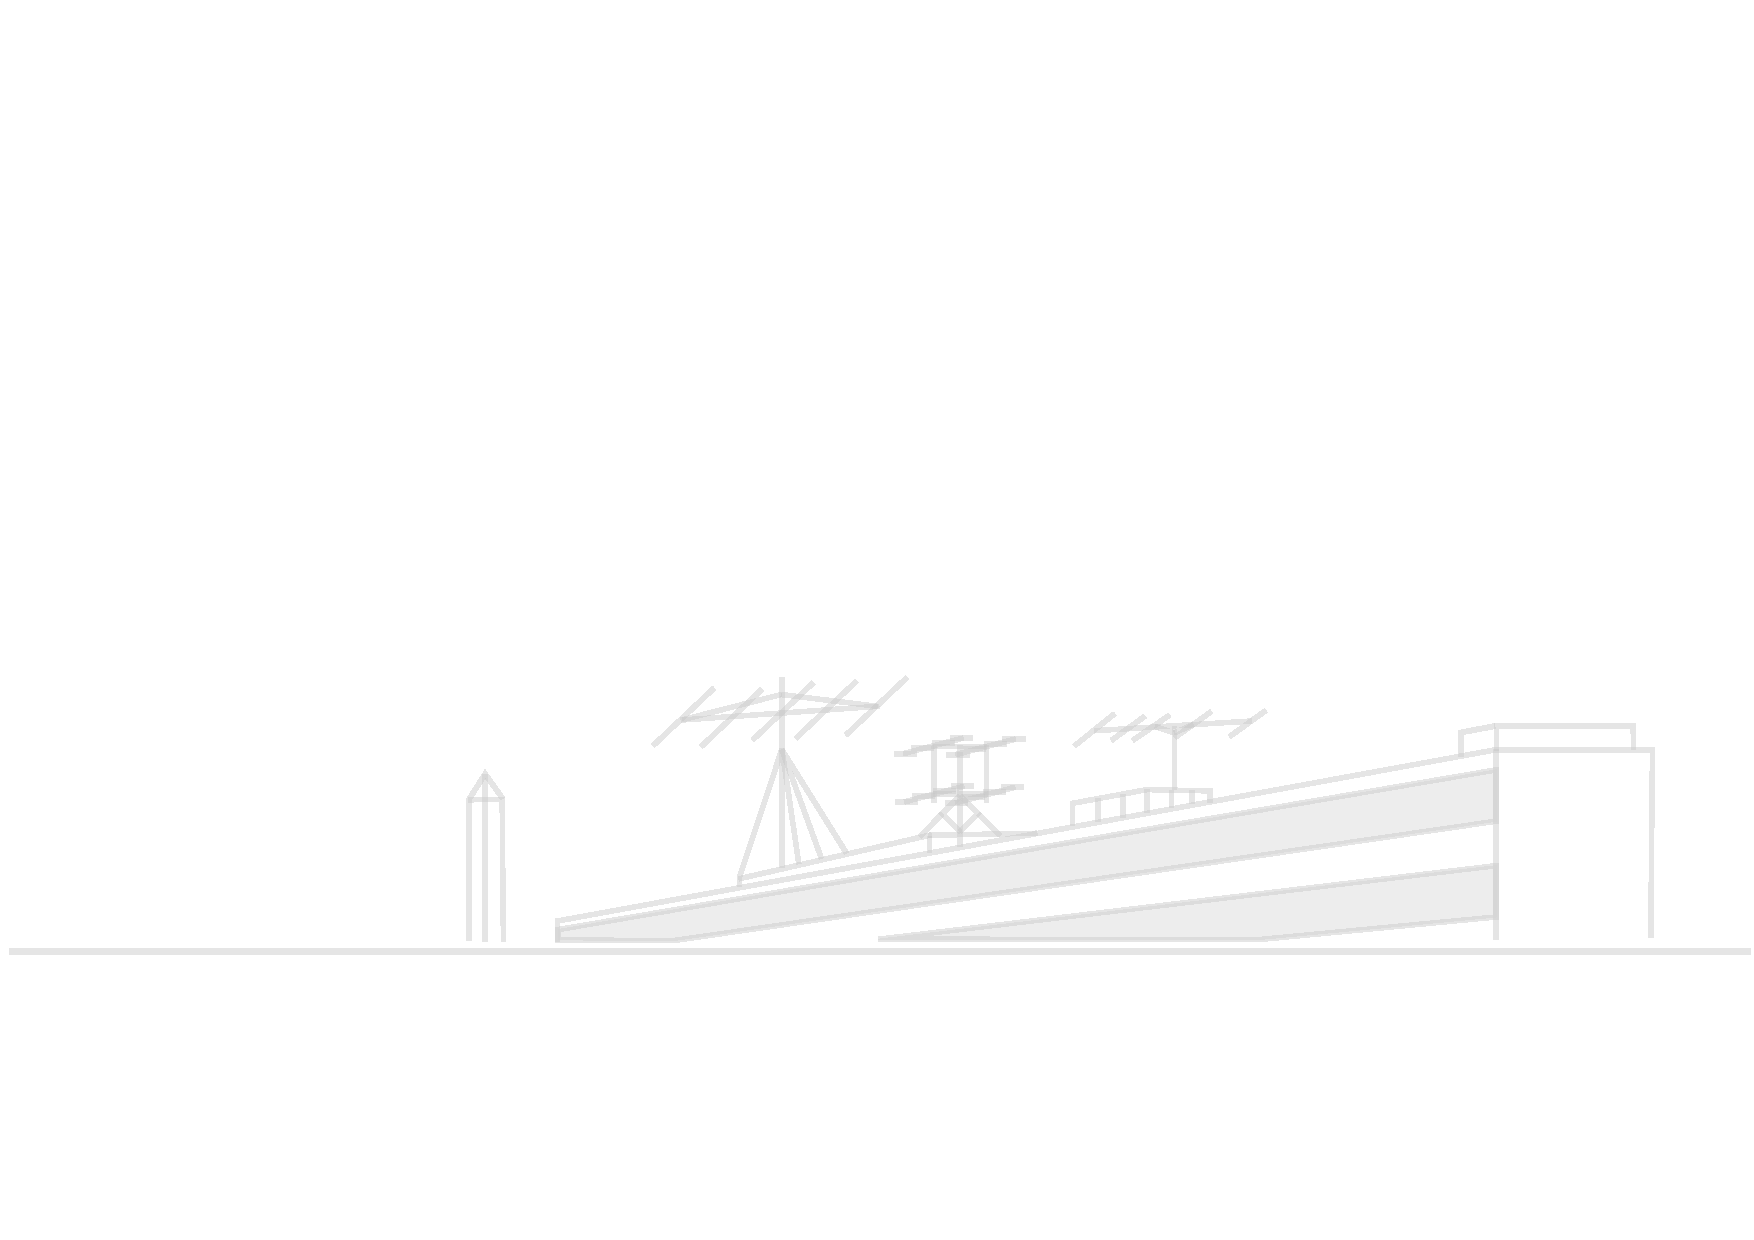
\includegraphics[width=17.8cm]{texdata/dk0tu_rooftop_background.pdf}
}

% Foliennummer einfügen
\setbeamertemplate{footline}[frame number]
%\setbeamertemplate{footline}{}

% Ändere das Zeichen vor jedem item
%\setbeamertemplate{itemize item}{\color{craneorange}$\blacktriangleright$}
%\setbeamertemplate{itemize subitem}{\color{craneorange}$\triangleright$}
%\setbeamertemplate{itemize subsubitem}{\color{craneorange}$\blacktriangleright$}

% Ändert die Blöcke 
\setbeamertemplate{blocks}[rounded][shadow=true]
% default | rounded [shadow=true|false]

%
% Eigene Kommandos
%

% Hack to get natbib and beamer working together. "The beamer user guide suggests
% that only the manual bibliography entry approach is supported"
% on some system it works out of the box, sometimes you need the hack :-(
% so check it --dl7bst
\ifdefined\newblock
    \relax
\else
    \newcommand{\newblock}{}
\fi

% \includedia command to generate png out of a dia file
% NEEDS installed dia and pdflatex option --shell-escape
\newcommand{\includedia}[1]{
    \immediate\write18{/usr/bin/dia #1.dia -e #1_diatmp.png -t png}
}

% RICHIG GROSSER FONT!
\newfont{\bigfont}{cmr10 at 144pt}
\newfont{\smallfont}{cmr10 at 8pt}

% Römische Ziffern
\makeatletter
\newcommand{\rmnum}[1]{\romannumeral #1}
\newcommand{\Rmnum}[1]{\expandafter\@slowromancap\romannumeral #1@}
\makeatother

% Schwarze Überschrift
%\setbeamercolor{frametitle}{fg=black}
%\setbeamercolor{title}{fg=black}

% Item- und Box-Farben
\definecolor{deepBlue}{HTML}{000066}
\setbeamercolor{itemize item}{fg=deepBlue}
\setbeamercolor{itemize subitem}{fg=deepBlue}
\setbeamercolor{description item}{fg=deepBlue}
\setbeamercolor{block title}{fg=deepBlue!100, bg=blue!15}
\setbeamercolor{block body}{fg=black, bg=blue!5}
\setbeamercolor{block title alerted}{fg=deepBlue, bg=red!75}
\setbeamercolor{block body alerted}{fg=black, bg=red!15}
\setbeamercolor*{block title example}{fg=blue!50, bg=blue!10}
\setbeamercolor*{block body example}{fg= blue, bg=blue!5}

%\setbeamercolor{section in head/foot}{parent=palette primary}
%\setbeamercolor{subsection in head/foot}{parent=palette secondary}
%\setbeamercolor{sidebar}{fg=darkblue,bg=yellow!90!orange}
%\setbeamercolor{title in sidebar}{fg=darkblue}
%\setbeamercolor{author in sidebar}{fg=darkblue}
%\setbeamercolor{section in sidebar}{fg=darkblue!10!black}
%\setbeamercolor{subsection in sidebar}{fg=darkblue!50!black}

% Titlepage Infos
\title{AFu-Kurs nach DJ4UF}
\author[DKØTU]{DKØTU\\ \footnotesize{Amateurfunkgruppe der TU Berlin}}
\institute[DKØTU]{\url{http://www.dk0tu.de} }

% PDF-Eigenschaften
\subject{DK0TU-Amateurfunkkurs nach DJ4UF}
\keywords{Amateurfunk Kurs HAM Radio Course CC-BY-NC-SA OpenSource TU Berlin DK0TU}

\subtitle{Technik A14: \\
  Digitaltechnik \\[2em]}
\date{Stand 22.02.2016}
 \begin{document}

\begin{frame}
    \titlepage
    \vfill
    \begin{center}
        \ccbyncsaeu\\
        {\tiny This work is licensed under the \em{Creative Commons Attribution-NonCommercial-ShareAlike 3.0 License}.}\\[0.5ex]
         \tiny Amateurfunkgruppe der Technische Universität Berlin (AfuTUB), DKØTU
         %\includegraphics[scale=0.5]{img/DK0TU_Logo.pdf}
    \end{center}
\end{frame}


\begin{frame}{Digitaltechnik}
  Die Digitaltechnik kennt nur zwei Zustände:
  \begin{description}
    \item[0] LOW
    \item[1] HIGH
  \end{description}
  Zwischenwerte, wie in der Analogtechnik, sind nicht vorhanden.\\[2em]
  In der Realität ist es eine Definitionssache, ab welcher Spannung ein Signal als LOW oder HIGH angesehen wird.
\end{frame}


\section{Transistor als Schalter}


\begin{frame}{Transistor als Schalter}
  \begin{columns}
    \column{.5\textwidth}
    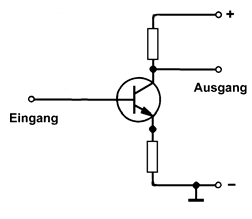
\includegraphics[width=\textwidth,height=.8\textheight,keepaspectratio]{a14/td401_simplified.png}\\
    {\tiny TD401 \hyperlink{refs}{\cite{bna}}}\\
    \column{.45\textwidth}
    \pause
    \begin{itemize}
      \item Transistor in Emitterschaltung
      \item Liegt am Eingang keine Spannung an, ist die Ausgangsspannung maximal
      \item Liegt am Eingang eine hohe Spannung an, wird die Ausgangsspannung minimal
      \item $\rightarrow$ \textbf{Inverter}
        \pause
      \item Es gibt in der Prüfung nur zwei Transistor-Logik-Schaltungen
      \item Zuerst ein Blick auf die Logikgatter
    \end{itemize}
  \end{columns}
\end{frame}

\subsection{NOT}

\begin{frame}{NOT}
  \begin{columns}
    \column[c]{.4\textwidth}
    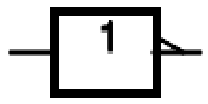
\includegraphics[width=\textwidth,height=.2\textheight,keepaspectratio]{a14/NOT_IEC.pdf}\\
    {\small Schaltsymbol IEC}\\
    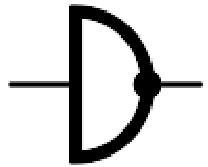
\includegraphics[width=\textwidth,height=.2\textheight,keepaspectratio]{a14/NOT_DIN.pdf}\\
    {\small Schaltsymbol DIN}\\
    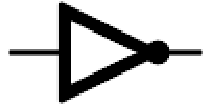
\includegraphics[width=\textwidth,height=.2\textheight,keepaspectratio]{a14/NOT_ANSI.pdf}\\
    {\small Schaltsymbol ANSI}
    \column{.55\textwidth}
    \begin{block}{Wahrheitstabelle}
      \begin{tabular}{c|c}
        \textbf{INPUT} & \textbf{OUTPUT} \\
        \textbf{A} & \textbf{NOT A} \\ \hline
        0 & 1 \\
        1 & 0 \\
      \end{tabular}
    \end{block}
  \end{columns}
\end{frame}

\subsection{AND}
\begin{frame}{AND}
  \begin{columns}
    \column[c]{.4\textwidth}
    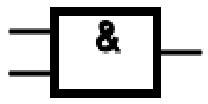
\includegraphics[width=\textwidth,height=.2\textheight,keepaspectratio]{a14/AND_IEC.pdf}\\
    {\small Schaltsymbol IEC}\\
    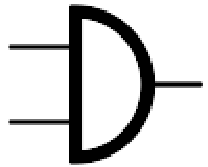
\includegraphics[width=\textwidth,height=.2\textheight,keepaspectratio]{a14/AND_DIN.pdf}\\
    {\small Schaltsymbol DIN}\\
    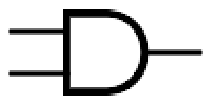
\includegraphics[width=\textwidth,height=.2\textheight,keepaspectratio]{a14/AND_ANSI.pdf}\\
    {\small Schaltsymbol ANSI}
    \column{.55\textwidth}
    \begin{block}{Wahrheitstabelle}
      \begin{tabular}{cc|c}
        \multicolumn{2}{c|}{\textbf{INPUT}} & \textbf{OUTPUT} \\
        \textbf{A} & \textbf{B} & \textbf{A AND B} \\ \hline
        0 & 0 & 0 \\
        0 & 1 & 0 \\
        1 & 0 & 0 \\
        1 & 1 & 1 \\
      \end{tabular}
    \end{block}
  \end{columns}
\end{frame}

\subsection{NAND}

\begin{frame}{NAND}
  \begin{columns}
    \column[c]{.4\textwidth}
    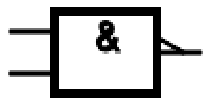
\includegraphics[width=\textwidth,height=.2\textheight,keepaspectratio]{a14/NAND_IEC.pdf}\\
    {\small Schaltsymbol IEC}\\
    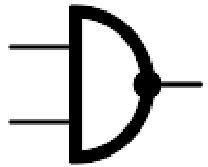
\includegraphics[width=\textwidth,height=.2\textheight,keepaspectratio]{a14/NAND_DIN.pdf}\\
    {\small Schaltsymbol DIN}\\
    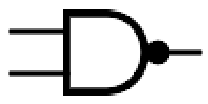
\includegraphics[width=\textwidth,height=.2\textheight,keepaspectratio]{a14/NAND_ANSI.pdf}\\
    {\small Schaltsymbol ANSI}
    \column{.55\textwidth}
    \begin{block}{Wahrheitstabelle}
      \begin{tabular}{cc|c}
        \multicolumn{2}{c|}{\textbf{INPUT}} & \textbf{OUTPUT} \\
        \textbf{A} & \textbf{B} & \textbf{A NAND B} \\ \hline
        0 & 0 & 1 \\
        0 & 1 & 1 \\
        1 & 0 & 1 \\
        1 & 1 & 0 \\
      \end{tabular}
    \end{block}
  \end{columns}
\end{frame}

\subsection{OR}

\begin{frame}{OR}
  \begin{columns}
    \column[c]{.4\textwidth}
    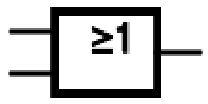
\includegraphics[width=\textwidth,height=.2\textheight,keepaspectratio]{a14/OR_IEC.pdf}\\
    {\small Schaltsymbol IEC}\\
    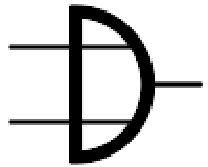
\includegraphics[width=\textwidth,height=.2\textheight,keepaspectratio]{a14/OR_DIN.pdf}\\
    {\small Schaltsymbol DIN}\\
    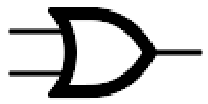
\includegraphics[width=\textwidth,height=.2\textheight,keepaspectratio]{a14/OR_ANSI.pdf}\\
    {\small Schaltsymbol ANSI}
    \column{.55\textwidth}
    \begin{block}{Wahrheitstabelle}
      \begin{tabular}{cc|c}
        \multicolumn{2}{c|}{\textbf{INPUT}} & \textbf{OUTPUT} \\
        \textbf{A} & \textbf{B} & \textbf{A OR B} \\ \hline
        0 & 0 & 0 \\
        0 & 1 & 1 \\
        1 & 0 & 1 \\
        1 & 1 & 1 \\
      \end{tabular}
    \end{block}
  \end{columns}
\end{frame}

\subsection{NOR}

\begin{frame}{NOR}
  \begin{columns}
    \column[c]{.4\textwidth}
    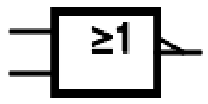
\includegraphics[width=\textwidth,height=.2\textheight,keepaspectratio]{a14/NOR_IEC.pdf}\\
    {\small Schaltsymbol IEC}\\
    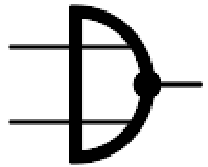
\includegraphics[width=\textwidth,height=.2\textheight,keepaspectratio]{a14/NOR_DIN.pdf}\\
    {\small Schaltsymbol DIN}\\
    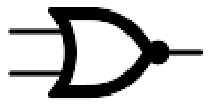
\includegraphics[width=\textwidth,height=.2\textheight,keepaspectratio]{a14/NOR_ANSI.pdf}\\
    {\small Schaltsymbol ANSI}
    \column{.55\textwidth}
    \begin{block}{Wahrheitstabelle}
      \begin{tabular}{cc|c}
        \multicolumn{2}{c|}{\textbf{INPUT}} & \textbf{OUTPUT} \\
        \textbf{A} & \textbf{B} & \textbf{A NOR B} \\ \hline
        0 & 0 & 1 \\
        0 & 1 & 0 \\
        1 & 0 & 0 \\
        1 & 1 & 0 \\
      \end{tabular}
    \end{block}
  \end{columns}
\end{frame}

\subsection{XOR}

\begin{frame}{XOR}
  \begin{columns}
    \column[c]{.4\textwidth}
    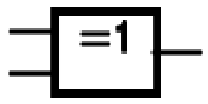
\includegraphics[width=\textwidth,height=.2\textheight,keepaspectratio]{a14/XOR_IEC.pdf}\\
    {\small Schaltsymbol IEC}\\
    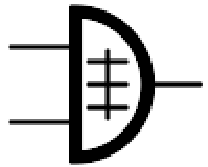
\includegraphics[width=\textwidth,height=.2\textheight,keepaspectratio]{a14/XOR_DIN.pdf}\\
    {\small Schaltsymbol DIN}\\
    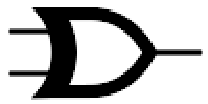
\includegraphics[width=\textwidth,height=.2\textheight,keepaspectratio]{a14/XOR_ANSI.pdf}\\
    {\small Schaltsymbol ANSI}
    \column{.55\textwidth}
    \begin{block}{Wahrheitstabelle}
      \begin{tabular}{cc|c}
        \multicolumn{2}{c|}{\textbf{INPUT}} & \textbf{OUTPUT} \\
        \textbf{A} & \textbf{B} & \textbf{A XOR B} \\ \hline
        0 & 0 & 0 \\
        0 & 1 & 1 \\
        1 & 0 & 1 \\
        1 & 1 & 0 \\
      \end{tabular}
    \end{block}
  \end{columns}
\end{frame}

\subsection{Fragen}

\begin{frame}
  \begin{tabular}{l||p{.8\textwidth}}\hline
    \textbf{TC703} & \textbf{Wie heißen die Grundbausteine in der Digitaltechnik} \\ \hline\hline
    A & (+)-Gatter (UND), (-)-Gatter (OR), NICHT-(+)-Gatter (NUND), NICHT-(-)-Gatter (NODER). \\ \hline
    B & UND-Gatter (UNG), ODER-Gatter (ORG), NICHT-UND-Gatter (NUNG), NICHT-ODER-Gatter (NORG). \\ \hline
    C & UND-Glied (UND), ODER-Glied (ODER), NICHT-UND-Glied (NUND), NICHT-ODER-Glied (NODER). \\ \hline
    D \only<2>\checkmark & UND-Glied (AND), ODER-Glied (OR), NICHT-UND-Glied (NAND), NICHT-ODER-Glied (NOR). \\ \hline
  \end{tabular}
\end{frame}

\begin{frame}
  \begin{scriptsize}
    \begin{tabular}{l||p{.8\textwidth}}\hline
      \textbf{TC705} & \textbf{Welche logische Grundschaltung stellt die folgende Transistorschaltung dar und wie arbeitet sie?}

      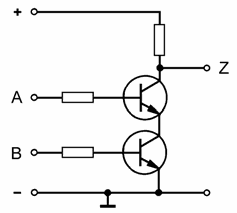
\includegraphics[width=.5\textwidth,height=.3\textheight,keepaspectratio]{a14/tc705.png}\\ \hline\hline
      A & Die Schaltung stellt ein OR-Gatter dar. Der Ausgang Z führt dann Nullpotential, wenn die Eingänge A und B mit der Betriebsspannung verbunden sind. In allen anderen Fällen führt der Ausgang Z die Betriebsspannung. \\ \hline
      B & Die Schaltung stellt ein NOR-Gatter [negiertes ODER-Gatter] dar. Der Ausgang Z führt dann die Betriebsspannung, wenn keiner der beiden Eingänge A oder B mit der Betriebsspannung verbunden ist. In allen anderen Fällen führt der Ausgang Z Nullpotential. \\ \hline
      C \only<2>\checkmark & Die Schaltung stellt ein NAND-Gatter [negiertes UND-Gatter] dar. Der Ausgang Z führt dann Nullpotential, wenn die Eingänge A und B mit der Betriebsspannung verbunden sind. In allen anderen Fällen führt der Ausgang Z die Betriebsspannung. \\ \hline
      D & Die Schaltung stellt ein AND-Gatter dar. Der Ausgang Z führt dann Betriebsspannung, wenn die Eingänge A und B mit der Betriebsspannung verbunden sind. In allen anderen Fällen führt der Ausgang Z Nullpotential. \\ \hline
    \end{tabular}
  \end{scriptsize}
\end{frame}

\begin{frame}
  \begin{scriptsize}
    \begin{tabular}{l||p{.8\textwidth}}\hline
      \textbf{TC706} & \textbf{Welche logische Grundschaltung stellt die folgende Transistorschaltung dar und wie arbeitet sie?}

      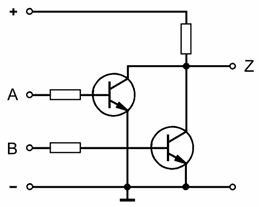
\includegraphics[width=.5\textwidth,height=.3\textheight,keepaspectratio]{a14/tc706.png}\\ \hline\hline
      A \only<2>\checkmark & Die Schaltung stellt ein NOR-Gatter [negiertes ODER-Gatter] dar. Der Ausgang Z führt dann die Betriebsspannung, wenn beide Eingänge A und B Nullpotential führen bzw. offen sind. In allen anderen Fällen führt der Ausgang Z Nullpotential. \\ \hline
      B & Die Schaltung stellt ein NAND-Gatter [negiertes UND-Gatter] dar. Der Ausgang Z führt dann Nullpotential, wenn die Eingänge A und B mit der Betriebsspannung verbunden sind. In allen anderen Fällen führt der Ausgang Z die Betriebsspannung. \\ \hline
      C & Die Schaltung stellt ein OR-Gatter dar. Der Ausgang Z führt dann Betriebsspannung, wenn die Eingänge A und B mit der Betriebsspannung verbunden sind. In allen anderen Fällen führt der Ausgang Z die Nullpotential. \\ \hline
      D & Die Schaltung stellt ein AND-Gatter dar. Der Ausgang Z führt dann Nullpotential, wenn die Eingänge A und B mit der Betriebsspannung verbunden sind. In allen anderen Fällen führt der Ausgang Z Betriebsspannung. \\ \hline
    \end{tabular}
  \end{scriptsize}
\end{frame}

\section{Zeit"-ablauf"-diagramme}
\begin{frame}{Zeitablaufdiagramme}
  \begin{columns}
    \column[c]{.45\textwidth}
    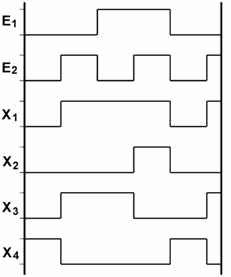
\includegraphics[width=\textwidth,height=.8\textheight,keepaspectratio]{a14/tc707.png}\\
    {\tiny TC707--TC709 \hyperlink{refs}{\cite{bna}}}
    \column[c]{.5\textwidth}
    \begin{itemize}
      \item zur Überprüfung digitaler Schaltungen
      \item an die Eingänge werden wechselnde Signale angelegt
      \item die Beobachtung des Ausgangs mit einem Speicheroszilloskop ergibt Rückschlüsse auf die verwendete Schaltung
    \end{itemize}
    \pause
    \begin{description}
      \item[$x_1\rightarrow$] \only<3>{OR}
      \item[$x_2\rightarrow$] \only<3>{AND}
      \item[$x_3\rightarrow$] \only<3>{XOR}
      \item[$x_4\rightarrow$] \only<3>{NOR}
    \end{description}
  \end{columns}
\end{frame}

\section{Logik"-schaltungen}
\begin{frame}{Logikschaltungen}
  \begin{columns}
    \column[c]{.45\textwidth}
    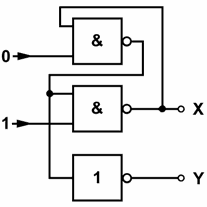
\includegraphics[width=\textwidth,height=.8\textheight,keepaspectratio]{a14/tc704.png}\\
    {\tiny TC704 \hyperlink{refs}{\cite{bna}}}
    \column[c]{.5\textwidth}
    \begin{itemize}
      \item Zusammenschaltung mehrerer Logikgatter
      \item Komplexe Aufgaben können bewältigt werden
      \item ``Programmieren in Hardware''
      \item Beispiele sind Schaltungen für Rechenoperationen, Flipflops oder Multiplexer
      \item Daraus lassen sich wiederum Datenspeicher, Zähler oder ganze Mikroprozessoren aufbauen
      \item \emph{Beispiel: \href{https://media.ccc.de/v/gpn14_-_5862_-__-_medientheater_-_201406211600_-_zuse_z22_-_lorenz_hanewinkel}{$\Rightarrow$ Lorenz Hanewinkel über die Konstruktion der Z22}}
    \end{itemize}
  \end{columns}
\end{frame}

\begin{frame}{Beispiel: R-S-Flipflop}
  \begin{columns}
    \column{.48\textwidth}
    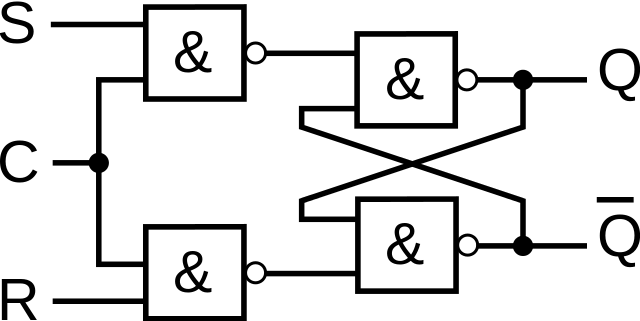
\includegraphics[width=\textwidth,height=.8\textheight,keepaspectratio]{a14/ISO-RS-FF-NAND-with-clock.png}\\
    {\tiny Logik-Schaltung eines getakteten RS-Flipflops aus vier NAND-Gattern \hyperlink{refs}{\cite{wp}}}
    \column{.48\textwidth}
    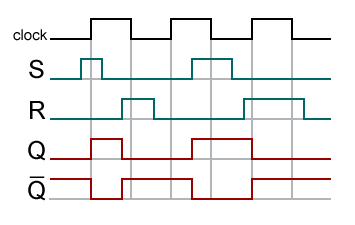
\includegraphics[width=\textwidth,height=.8\textheight,keepaspectratio]{a14/SR_latch_impulse_diagram.png}\\
    {\tiny Impulsdiagramm (SR-Latch) \hyperlink{refs}{\cite{wp}}}
  \end{columns}
\end{frame}


\begin{frame}
  \begin{tabular}{l||p{.8\textwidth}}\hline
    \textbf{TC704} & \textbf{Welche der Aussagen trifft für diese Schaltung zu?}

    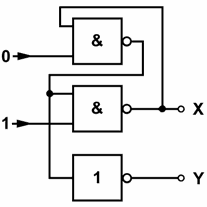
\includegraphics[width=.6\textwidth,height=.6\textheight,keepaspectratio]{a14/tc704.png}\\ \hline\hline
    A & X=1 und Y=0 \\ \hline
    B \only<2>\checkmark & X=0 und Y=0 \\ \hline
    C & X=1 und Y=1 \\ \hline
    D & X=0 und Y=1 \\ \hline
  \end{tabular}
\end{frame}

\section{Pegel"-anpassung}
\begin{frame}{Pegelanpassung}
  \begin{itemize}
    \item nicht alle ICs oder Schaltungen liefern 0 und +5V
    \item durch entsprechende Pegelwandler können die Pegel normiert werden
    \item \emph{wird in der Prüfung nicht gefragt, aber nützliches Wissen, wenn der 5V-Ausgang des Arduino den 3,3V-GPIO am Raspberry Pi brät\ldots}
  \end{itemize}
\end{frame}

\begin{frame}
  \begin{tabular}{l||p{.8\textwidth}}\hline
    \textbf{TC710} & \textbf{In welchem Versorgungsspannungsbereich können CMOS-ICs betrieben werden?} \\ \hline\hline
    A \only<2>\checkmark & $+3V$ bis $+15V$ \\ \hline
    B & $+2,5V$ bis $+5,5V$ \\ \hline
    C & $\pm2,5V$ bis $\pm5,5V$ \\ \hline
    D & $\pm5V$ \\ \hline
  \end{tabular}
\end{frame}

\section{Zahlensysteme}

\subsection{Dual}
\begin{frame}{Dualzahlen}
  \begin{exampleblock}{}
    {\Large``There are only 10 types of people in the world:\\
    those who understand binary, and those who don't.''}\\[1em]
    \hspace*\fill{\small--- Mathematical joke}
  \end{exampleblock}
\end{frame}

\begin{frame}{Dualzahlen}
  \begin{columns}
    \column{.5\textwidth}
    \begin{tabular}{r|c|r}
      \textbf{Binär} & \textbf{Potenz} & \textbf{Dezimal} \\ \hline
      0 & $0$ & 0 \\
      1 & $2^0$ & 1 \\
      10 & $2^1$ & 2 \\
      11 & $2^1+2^0$ & 3 \\
      100 & $2^2$ & 4 \\
      101 & $2^2+2^0$ & 5 \\
      110 & $2^2+2^1$ & 6 \\
      111 & $2^2+2^1+2^0$ & 7 \\
    \end{tabular}
    \column{.5\textwidth}
    \begin{tabular}{r|c|r}
      \textbf{Binär} & \textbf{Potenz} & \textbf{Dezimal} \\ \hline
      0 & $0$ & 0 \\
      1 & $2^0$ & 1 \\
      10 & $2^1$ & 2 \\
      100 & $2^2$ & 4 \\
      1000 & $2^3$ & 8 \\
      10000 & $2^4$ & 16 \\
      100000 & $2^5$ & 32 \\
      1000000 & $2^6$ & 64 \\
      10000000 & $2^7$ & 128 \\
      100000000 & $2^8$ & 256 \\
      1000000000 & $2^9$ & 512 \\
      10000000000 & $2^{10}$ & 1024 \\
    \end{tabular}
  \end{columns}
\end{frame}

\begin{frame}
  \begin{tabular}{l||p{.8\textwidth}}\hline
    \textbf{TC722} & \textbf{Welche dezimalen Werte haben die Stellen der Dualzahl 111111 von links nach rechts?} \\ \hline\hline
    A & 1, 2, 4, 8, 16, 32 \\ \hline
    B \only<2>\checkmark & 32, 16, 8, 4, 2, 1 \\ \hline
    C & 65536, 256, 16, 4, 2, 1 \\ \hline
    D & 100000, 10000, 1000, 100, 10, 1 \\ \hline
  \end{tabular}
\end{frame}

\begin{frame}
  \begin{tabular}{l||p{.8\textwidth}}\hline
    \textbf{TC720} & \textbf{Berechnen Sie den dezimalen Wert der 8-Bit-Dualzahl 10001110. Die Dezimalzahl lautet} \\ \hline\hline
    A & 78. \\ \hline
    B \only<2>\checkmark & 142. \\ \hline
    C & 156. \\ \hline
    D & 248. \\ \hline
  \end{tabular}
\end{frame}


\subsection{Hexadezimal}
\begin{frame}{Hexadezimalzahlen}
  \begin{columns}
    \column{.5\textwidth}
    \begin{tabular}{r|r}
      \textbf{Hexadezimal} & \textbf{Dezimal} \\ \hline
      0 & 0 \\
      1 & 1 \\
      2 & 2 \\
      $\vdots$ & $\vdots$ \\
      9 & 9 \\
      A & 10 \\
      B & 11 \\
      C & 12 \\
      D & 13 \\
      E & 14 \\
      F & 15 \\
    \end{tabular}
    \column{.5\textwidth}
    \begin{tabular}{r|r}
      \textbf{Hexadezimal} & \textbf{Dezimal} \\ \hline
      10 & 16 \\
      11 & 17 \\
      $\vdots$ & $\vdots$ \\
      1F & 31 \\
      20 & 32 \\
      21 & 33 \\
      $\vdots$ & $\vdots$ \\
      FE & 254 \\
      FF & 255 \\
    \end{tabular}
  \end{columns}
\end{frame}

\begin{frame}
  \begin{tabular}{l||p{.8\textwidth}}\hline
    \textbf{TC721} & \textbf{Wie lautet der dezimale Wert der zweistelligen Hexadezimalzahl 1A? Die Dezimalzahl lautet} \\ \hline\hline
    A & 16. \\ \hline
    B & 11. \\ \hline
    C \only<2>\checkmark & 26. \\ \hline
    D & 160. \\ \hline
  \end{tabular}
\end{frame}


\renewcommand{\refname}{Referenzen}

\hypertarget{refs}{}
\textcolor{white}{} \\ %\vspace{} geht nicht
\Large Referenzen/Links
\footnotesize

\begin{thebibliography}{}
  \bibitem{darc}  DARC Online-Lehrgang Lektion A14:\\
    \url{https://www.darc.de/der-club/referate/ajw/lehrgang-ta/a14/}
  \bibitem{wm}  Wikimedia:\\
    \href{https://commons.wikimedia.org/wiki/Logic_gates_unified_symbols}{Logic Gates Unified Symbols, Public Domain}\\
  \bibitem{wp}    Wikipedia - Die freie Enzyklopädie:\\
    \href{https://de.wikipedia.org/wiki/Flipflop}{Flipflop}\\
  \bibitem{bna}   Fragenkatalog Bundesnetzagentur Technik Klasse A:\\
    \url{https://www.bundesnetzagentur.de/SharedDocs/Downloads/DE/Sachgebiete/Telekommunikation/Unternehmen_Institutionen/Frequenzen/Amateurfunk/Fragenkatalog/TechnikFragenkatalogKlasseAf252rId9014pdf.pdf?__blob=publicationFile&v=3}
\end{thebibliography}

% Hier könnte noch eine Kontaktfolie stehen

\end{document}

